\section{Introduction (2~p)}\label{sec:introduction}

% The authors acknowledge support by the state of Baden-Württemberg through \href{https://www.bwhpc.de/}{bwHPC}.

\section{Related Work (3~p)}\label{sec:related-work}

\textbf{Trade Classification in Option Markets}

While classical trade classification algorithms are extensively tested in the stock markets (e.g., \textcite{chakrabartyTradeClassificationAlgorithms2012}; \textcite{odders-whiteOccurrenceConsequencesInaccurate2000}), few works have examined trade classification in option markets.

\textcite[\pno~882f.]{savickasInferringDirectionOption2003} are the first to compare the tick rule, quote rule, the Lee and Ready algorithm and the EMO rule for options traded at the CBOE. The data set spans a period from July 3, 1995 - December 31, 1995 consisting of $869{,}217$ matched trades. The authors report the highest accuracies for the quote rule ($78.98~\%$) and find that all rules perform worst when applied to index options. In general, the trade classification rules exhibit significantly lower classification accuracies on options data than with stock data, urging the need for improved classifiers.

The most exhaustive study is the one of \textcite[\pno~1f.]{grauerOptionTradeClassification2022}.  The authors test the accuracy of the classical quote rule and tick rule, and hybrids thereof on two large-scale data sets spanning a period from 2005 - 2017. Consistently for options traded at the ISE and CBOE classical rules like the popular Lee and Ready algorithm only achieve accuracies of $62.53~\%$ or $62.03~\%$ and are thus significantly smaller than in the stock market. In line with the research of  \textcite[\pno~886]{savickasInferringDirectionOption2003}, the reported accuracies are inversely proportional to the rule's reliance on past transaction prices. In particular, the tick rule performs worst with accuracies marginally different from a random guess. Overall, the reported success rates deteriorate between both studies and over time. As a remedy, \textcite[\pno~14f.]{grauerOptionTradeClassification2022} introduce two additional rules based on the trade and quote sizes. The \textit{depth rule} is an alternative to the tick rule for classifying mid spread trades in the Lee and Ready algorithm and EMO rule. It assigns the aggressor of the trade based on the depth at the bid or ask. Together with the \textit{trade size rule}, their second rule, which classifies trades with a trade size matching the size of the bid or ask quote, can substantially improve the performance of classical algorithms. The ensemble of rules achieves an accuracy between $73~\%$ and $75~\%$ surpassing previous rules by more than $10~\%$, at the cost of data efficiency.

The work of \textcite{grauerOptionTradeClassification2022} is important in two ways. First, the data set is identical to ours, which enables a fair comparison between classical rules and machine learning-based predictors. Second, their stacked combinations of the trade size rule, depth rule, and common trade classification algorithms achieve state-of-the-art performance in option trade classification and are thus a rigorous benchmark.

\textbf{Trade classification using machine learning}

\textcite[\pno~5]{rosenthalModelingTradeDirection2012} bridges the gap between classical trade classification and machine learning by fitting a logistic regression model on lagged and unlagged predictors inherent to the tick rule, quote rule, and EMO algorithm, as well as a sector-specific and a time-specific term. Instead of using the rule's discretized outcome as a feature, \textcite[\pno~481f.]{rosenthalModelingTradeDirection2012} models the rules through so-called information strength functions. The proximity to the quotes, central to the EMO algorithm, is thus modelled by a proximity function. Likewise, the information strength of the quote and tick rule is estimated as the log return between the trade price and the midpoint or the previous trade price. However, it only improves the accuracy of the EMO algorithm by a marginal $2~\%$ for Nasdaq stocks and $1.1~\%$ for NYSE stocks \textcite[\pno~15]{rosenthalModelingTradeDirection2012}. Our work aims to improve the model by exploring non-linear estimators and minimizing data modelling assumptions.

The work of \textcite[\pno~481f.]{blazejewskiLocalNonParametricModel2005} compares a $k$-nearest neighbour classifier against logistic regression, as well as simple heuristics like the majority vote over past trades for signing trades at the Australian stock exchange. Their results indicate that the parametric $k$-nearest neighbour classifier improves upon a linear logistic regression in terms of classification accuracy, even when trained on fewer features. The work is unique from the remaining works about feature set definition. Notably, \textcite[\pno~3]{blazejewskiLocalNonParametricModel2005} use no quote or trade prices, but rather the order book volumes, trade sizes, and past trade signs for classification. No accuracies for classical trade signing rules are reported, which impedes a comparison across different works. In line with their results, we focus on non-linear models in the form of gradient boosting and transformers. Additionally, our paper addresses the mentioned shortcomings by benchmarking against state-of-the-art trade classification rules. We share the idea of using the trade size, as well as the bid and ask sizes for classification for some of our feature sets, but greedily predict using non-historic features.

Closest to our work is a publication of \textcite[\pno~1f.]{ronenMachineLearningTrade2022}. Therein, the authors compare a selection of machine learning algorithms against classical trade signing rules in the bond and stock market. Their comparison is the first to consider both logistic regression, a random forest, as well as feed-forward networks. Over a wide range of feature sets the tree-based ensemble consistently outperforms by out-of-sample accuracy the tick rule and Lee and Ready algorithm, as well as all remaining machine learning models. For the TRACE and ITCH data set, their best variant of the random forest outperforms the tick rule by $8.3~\%$ and $3.3~\%$, respectively \autocite[\pno~57]{ronenMachineLearningTrade2022}. Whilst the superiority of random forests is consistent for the bond and equity market, fitted classifiers do not transfer across markets, as diminishing accuracies for the transfer learning by model transfer indicate.

The results convincingly demonstrate the potential of machine learning, i.e., of tree-based ensembles, for trade classification. Yet, the comparability of the results is limited by the classifier's reliance on additional features beyond quote and price data. Albeit, \textcite[\pno~4]{ronenMachineLearningTrade2022} consider a wide range of approaches, their selection leaves the latest advancements in artificial neural networks and ensemble learning aside and is mainly guided by computational constraints. Even if the focus is on standard techniques, the unclear research agenda concerning model selection, tuning, and testing hampers the transferability of their results to the yet unstudied option market.

In summary, machine learning has been applied successfully in the context of trade classification. To the best of our knowledge, no previous work perform machine learning-based classification in the options markets.

\newpage
\section{Rule-Based Approaches (5.5~p)}\label{sec:rule-based-approaches}


% The following section introduces common rules for signing option trades. We start by introducing the classical quote and tick rule and continue with the more recent depth and trade size rule. In section \ref{hybrid-rules} we combine some rules from section \ref{basic-rules} to hybrids thereof. We conclude this chapter by drawing a connection to ensemble learning.

\subsection{Basic Rules (3~p)}\label{sec:basic-rules}

% Starting with the quote rule, we describe the most common rule for signing option trades, which can either be used as-is or joint in more complex rules.

\subsubsection{Quote Rule (0.75~p)}\label{sec:quote-rule}

The quote rule compares the trade price against the corresponding quotes at the time of the trade. If the trade price $P_{i,t}$ is above the midpoint of the bid-ask spread, denoted by $m_{i,t}$, the trade is classified as a buy and if it is below the midpoint, as a sell \autocite[][p.41]{harrisDayEndTransactionPrice1989}. Thus, the classification rule is formally given by:

\begin{equation}
  \text{Trade}_{i,t}=
  \begin{cases}
    0, & \text{if}\ P_{i, t}>m_{i, t}  \\
    1, & \text{if}\ P_{i, t}<m_{i, t}. \\
    %\\\texttt{[NAN]}, & \text{otherwise} %
  \end{cases}
\end{equation}

By definition, the quote rule cannot classify trades at the midpoint of the quoted spread. \textcite[][241]{hasbrouckTradesQuotesInventories1988} discusses multiple alternatives for signing mid-spread trades based on the subsequent quotes, contemporaneous, or the subsequent transaction. However, the most common approach to overcome this limitation is, to combine the quote rule with other approaches, such as the tick rule, into an ensemble.

The quote rule requires to match \emph{one} bid and ask quotes with each trade based on a timestamp. Due to the finite resolution of the dataset's timestamps and active markets, multiple quote changes can co-occur at the time of the trade, some of which, are actually after the trade. As such, it remains unclear which quote to consider in trade classification, and a \emph{quote timing technique} must be employed. Empirically, \textcite[][p.1{,}765]{holdenLiquidityMeasurementProblems2014} observe, that the most common choice is to use the last quote by order from the time increment (e.g., the second) before the trade.

In contrast to the tick rule, the quote rule requires both trade price and quote data, and is thus less data efficient. The reduced dependence on past transaction prices and the focus on quotes has nonetheless positively impacted classification accuracies in option markets, as the studies of \textcite[][p.886]{savickasInferringDirectionOption2003} and \textcite[][p.3]{grauerOptionTradeClassification2022} reveal. Especially, if trade classification is performed on the NBBO.


\subsubsection{Tick Test (0.75~p)}\label{sec:tick-test}



\subsubsection{Depth Rule (0.75~p)}\label{sec:depth-rule}

As the chapter tick test unveils, the tick rule yields significantly lower success rates than the quote rule. For midspread trades, that can otherwise not be classified by the advantageous quote rule,\textcite[][p.14]{grauerOptionTradeClassification2022} propose the \emph{depth rule}.

The depth rule infers the trade initiator from the quoted size at the best bid and ask. Based on the observation that an exceeding bid or ask size relates to higher liquidity on one trade side, trades are classified as a buy for a larger ask size and sell for a higher bid size \textcite[][p. 14]{grauerOptionTradeClassification2022}.

Let $\tilde{A}_{i,t}$ denote the quoted size of the ask and $\tilde{B}_{i,t}$ the size of the bid. The depth rule is formally given by:

\begin{equation}
  \text{Trade}_{i,t}=
  \begin{cases}
    0, & \text{if}\ P_{i, t} = m_{i, t}\ \text{and}\ \tilde{A}_{i,t} < \tilde{B}_{i,t}  \\
    1, & \text{if}\ P_{i, t} = m_{i, t}\ \text{and}\ \tilde{A}_{i,t} > \tilde{B}_{i,t}. \\
  \end{cases}
  \label{eq:depth-rule}
\end{equation}

As shown in Equation \ref{eq:depth-rule}, the depth rule classifies midspread trades only, if the ask size is different from the bid size, as the ratio between the ask and bid size is the sole criterion for inferring the trade's aggressor. Due to these restrictive conditions, the depth rule can only sign a small fraction of all trades and is best stacked with others rules.

Like the quote rule, the depth rule has additional dependencies on quote data. Despite being applied to midspread trades only, \textcite[][p.4]{grauerOptionTradeClassification2022} report an improvement in the overall accuracy $1.2~\%$ for the CBOE data set and by $0.8~\%$ on the ISE sample merely through the depth rule. The rule has not yet been tested in other markets.


\subsubsection{Trade Size Rule (0.75~p)}\label{sec:trade-size-rule}

% \begin{algorithm}

%   % input/ouput names
%   \SetKwInOut{Input}{Input}
%   \SetKwInOut{Output}{Output}
%   \SetKw{And}{\textbf{and}}
%   % caption
%   % TODO: set input and output: e. g., $\hat{e} \leftarrow$ layer_norm $(e \mid \gamma, \beta)$
%   \caption{$\operatorname{\mathtt{tradesize}}(t_i, a_i, b_i)$ \label{sec:alg:tradesize-rule}}

%   \Input{%
%     $\tilde{t}_i$ trade size at $i$, $\tilde{a}_i$ ask size at $i$, and $\tilde{b}_i$ bid size at $i$.
%   }
%   \Output{%
%     $o_i \in\{-1,1\}$ trade initiator for $i$-th trade.
%   }

%   \BlankLine % blank line for spacing

%   \uIf{$\tilde{a}_i = \tilde{t}_i$ \And $\tilde{b}_i \neq \tilde{t}_i$}{%
%     \Return{$o_i =-1$}
%   }
%   \uElseIf{$\tilde{b}_i = \tilde{t}_i$ \And $\tilde{a}_i \neq \tilde{t}_i$}{%
%     \Return{$o_i =1$}
%   }
%   \uElse{%
%     \Return \tcc*{apply secondary rule}
%   }
% \end{algorithm}


\subsection{Hybrid Rules (2.5~p)}\label{sec:hybrid-rules}

\subsubsection{Lee and Ready Algorithm (1 p)}\label{sec:lee-and-ready-algorithm}
% '
% \begin{algorithm}

%   % input/ouput names
%   \SetKwInOut{Input}{Input}
%   \SetKwInOut{Output}{Output}

%   % caption
%   % TODO: set input and output: e. g., $\hat{e} \leftarrow$ layer_norm $(e \mid \gamma, \beta)$
%   \caption{$\operatorname{\mathtt{lee-ready}}{(t_i, a_i, b_i)}$ \label{sec:alg:lee-ready-algorithm}}

%   \Input{%
%     $t_i$ trade price at $i$, $a_i$ ask price at $i$, and $b_i$ bid price at $i$.
%   }
%   \Output{%
%     $o_i \in\{-1,1\}$ trade initiator at $i$. \\
%   }

%   \BlankLine % blank line for spacing

%   % start of the pseudocode
%   $m_i \leftarrow \frac{1}{2}(a_i + b_i)$ \tcc*{mid spread at $i$}

%   \For{$1, \cdots, I$}{
%     \uIf{$t_i > m_i$}{
%       \Return{$o_i = 1$}
%     }
%     \uElseIf{$t_i < m_i$}{
%       \Return{$o_i = -1$}
%     }
%     \Else{
%       \Return{$o_i = \operatorname{\mathtt{tick}}{(t_i, a_i, b_i)}$} \tcc*{see Section \ref{sec:tick-test}.}
%     }
%   } % end for i
%   % TODO: set input and output params
% \end{algorithm}

% \subsubsection{Reverse Lee and Ready
%   Algorithm (0.5~p)}\label{sec:reverse-lee-and-ready-algorithm}

\subsubsection{Ellis-Michaely-O'Hara
  Rule (0.75~p)}\label{sec:ellis-michaely-ohara-rule}

% \begin{algorithm}

%   % input/ouput names
%   \SetKwInOut{Input}{Input}
%   \SetKwInOut{Output}{Output}

%   % caption
%   % TODO: set input and output: e. g., $\hat{e} \leftarrow$ layer_norm $(e \mid \gamma, \beta)$
%   \caption{$\operatorname{\mathtt{emo}}$ \label{sec:alg:emo-rule}}

%   \Input{%
%     $t_i$ trade price at $i$, $a_i$ ask price at $i$, and $b_i$ bid price at $i$.
%   }
%   \Output{%
%     $o_i \in\{-1,1\}$ trade initiator at $i$.
%   }

%   \BlankLine % blank line for spacing

%   % start of the pseudocode
%   \For{$1, \cdots, I$}{
%     \uIf{$t_i = a_i$}{
%       \Return{$o_i = 1$}
%     }
%     \uElseIf{$t_i = b_i$}{
%       \Return{$o_i = -1$}
%     }
%     \Else{
%       \Return{$o_i = \operatorname{\mathtt{tick}}{(t_i, a_i, b_i)}$} \tcc*{see Section \ref{sec:tick-test}.}
%     }
%   } % end for i
%   % TODO: set input and output params
% \end{algorithm}

\subsubsection{Chakrabarty-Li-Nguyen-Van-Ness
  Method (0.75~p)}\label{sec:chakarabarty-li-nguyen-van-ness-method}

\newpage
\section{Supervised Approaches (12~p)}\label{sec:supervised-approaches}

\subsection{Selection of Approaches (2~p)}\label{sec:selection-of-approaches}

\subsection{Gradient Boosted Trees (2~p)}\label{sec:gradient-boosted-trees}

\subsubsection{Decision Tree (0.5~p)}\label{sec:decision-tree}

% A decision tree splits the feature space $\mathbb{R}^m$ into several disjoint regions $R$ through a sequence of recursive splits. A single split leads to two new sub-regions for a binary decision tree, whose shape depends on the attribute used for splitting and the previously performed splits. The tree is grown in size until a minimum threshold for the number of samples within a node or some other stopping criterion applies \autocite{breimanClassificationRegressionTrees2017}.
% Trees can be utilised for classification and regression tasks. Our introduction focuses on the regression setting only.

% A region corresponds to a node in the tree. For each terminal node of the tree or unsplit region, the response variable $f(x)$ is constant \autocite{breimanClassificationRegressionTrees2017}. For a tree with $M$ regions, the response for $x$ can be modelled as
% $$
%   f(x)=\sum_{m=1}^{M} \gamma_{m} \mathbbm{1}\left(x \in R_{m}\right),
% $$
% with $\mathbbm{1}$ being the indicator function for region conformance and $\gamma_m$ being the region's constant \autocite{hastietrevorElementsStatisticalLearning2009}. In the regression case, $\gamma_m$ is simply the average overall response variables of this particular region. As $\gamma_m$ is shared among all samples within the region, the estimates of the tree are similar to a histogram approximating the true regression surface.

% So far, it remains open how the best split can be found. The best split is where the deviation of all regions estimates and the true response variables diminishes. Over the entire tree, this error can be captured in the \gls{SSE} given by

% $$
%   E(M)=\frac{1}{N} \sum_{m \in M} \sum_{i \in R_m}\left(y_{i}-f(x_i)\right)^{2},
% $$

% which is subsequently minimized \autocite{breimanClassificationRegressionTrees2017}. Following \textcite{breimanClassificationRegressionTrees2017} we scan all combinations of possible $m$ and potential split values $s$ and choose the split, that leads to the largest improvement in the error of the child nodes compared to their parent node $E(m)$:

% $$
%   \Delta E(s, m)=E(m)-E\left(m_{l}\right)-E\left(m_{r}\right).
% $$


% Trivially, growing deeper trees leads to an improvement in the \gls{SSE}. Considering the extreme, where each sample is in its region, the tree would achieve the highest fit but perform poorly on unseen data. For trees that generalise, \textit{cost complexity pruning} procedures are employed. If pruned, their ability to capture non-linearities and adaptability to numerical and categorical data makes trees a flexible estimator.


\subsubsection{Gradient Boosting
  Procedure (1.5 p)}\label{sec:gradient-boosting-procedure}

%   One approach that aims to reduce the bias is \textit{gradient boosting}, which was popularised for regression by \textcite{friedmanGreedyFunctionApproximation2001}. Gradient boosting sequentially combines the approximations of several over-simplified models (so-called
%   \textit{weak-learners}) to an ensemble estimate. Shallow decision trees are commonly used weak learners.

%   The following introduction is adapted from \textcite{hastietrevorElementsStatisticalLearning2009}. For a \textit{boosted tree} several decision trees are combined through summation:

%   $$
%     f_{M}(x)=\sum_{m=1}^{M} T\left(x ; \Theta_{m}\right).
%   $$

%   Here, $M$ sets the number of iterations or trees being built. Instead of fitting trees directly to the data, the model in the $m$-th iteration is fitted to the residuals of the previous model. In this greedy approach, previously built trees remain unaltered while being the foundations for trees in later iterations.

%   At each iteration, one seeks to find the optimal parameter set $\Theta_{m}=\left\{R_{j m}, \gamma_{j m}\right\}_{1}^{J_{m}}$ for the $m$-th iteration, that minimizes the loss $\mathcal{L}$ between the true value and the composite prediction from the current model $f_{m-1}\left(x_{i}\right)$ and the tree, updating the residuals:

%   \begin{equation}
%     \label{eq:boosting-min-loss}
%     \hat{\Theta}_{m}=\arg \min _{\Theta_{m}} \sum_{i=1}^{N} \mathcal{L}\left(y_{i}, f_{m-1}\left(x_{i}\right)+T\left(x_{i} ; \Theta_{m}\right)\right).
%   \end{equation}

%   A common loss function for regression is the \textit{squared error loss}, which can be solved analytically by taking the derivative and setting it equal to zero. The predictions of a tree $T\left(x_{i}; \Theta_{m}\right)$, that yields the maximum decrease of Equation \ref{eq:boosting-min-loss} are similar to the components of the \textit{negative gradient descent}. However, the major drawback is that the gradient is only defined for data points $x_i$ seen during training, contradicting the creation of a generalising model $f_{M}(x)$. A more robust approach can be found in \textit{gradient boosting}.

%   Focusing only on the update step, which is executed $m = 1,\ldots, M$-times, \textit{gradient boosting} starts by calculating the negative gradient of the loss between the observed value for the $i$-th sample and its current predicted value:
%   $$
%     r_{i m}=-{\left[\frac{\partial \mathcal{L}\left(y_{i}, f\left(x_{i}\right)\right)}{\partial f\left(x_{i}\right)}\right]}_{f=f_{m-1}}.
%   $$
%   The components of the negative gradient are referred to as \textit{pseudo residuals}. Subsequently, a regression tree is then fit on these pseudo residuals. The $m$-th regression tree contains $J$ terminal regions denoted by $R_{j m}, j=1,2, \ldots, J_{m}$. The predicted estimate $\gamma_{j,m}$ for the $j$-th region is obtained by minimising a loss such as the squared loss:

%   $$
%     \gamma_{j m}=\arg \min _{\gamma} \sum_{x_{i} \in R_{j m}} \mathcal{L}\left(y_{i}, f_{m-1}\left(x_{i}\right)+\gamma\right).
%   $$

%   Recall from Section
%    \ref{sec:decision-tree} that the estimate $\gamma_{jm}$ is constant for the entire region. As before, the best estimate is simply the average of all residuals within a region.

%   An improved estimate for $x$ is calculated from the previous estimate by adding the trees fitted on the residuals, as shown in Equation \ref{eq:boosting-final-estimate}. The latter moves the prediction towards the greatest descent and thus improves the overall prediction:

%   \begin{equation}\label{eq:boosting-final-estimate}
%     f_{m}(x)=f_{m-1}(x)+\nu \sum_{j=1}^{J_{m}} \gamma_{j m} \mathbbm{1}\left(x \in R_{j m}\right).
%   \end{equation}

%   Only proportional steps towards the negative gradient are taken to prevent overfitting. The pace is controlled by the learning rate $\nu \in (0, 1]$. While a small learning rate slows down learning, it allows more differently shaped trees to attack the residuals. After $M$ iterations we obtain the final estimate calculated as: $\hat{f}(x)=f_{M}(x)$.


% \subsubsection{Adaptions for Probabilistic
%   Classification (0.5~p)}\label{sec:adaptions-for-probablistic-classification}

\subsection{Transformer Networks}\label{sec:transformer-networks}

\subsubsection{Architectural Overview}\label{sec:architectural-overview}

\begin{landscape}
  \begin{figure}
    \begin{center}
      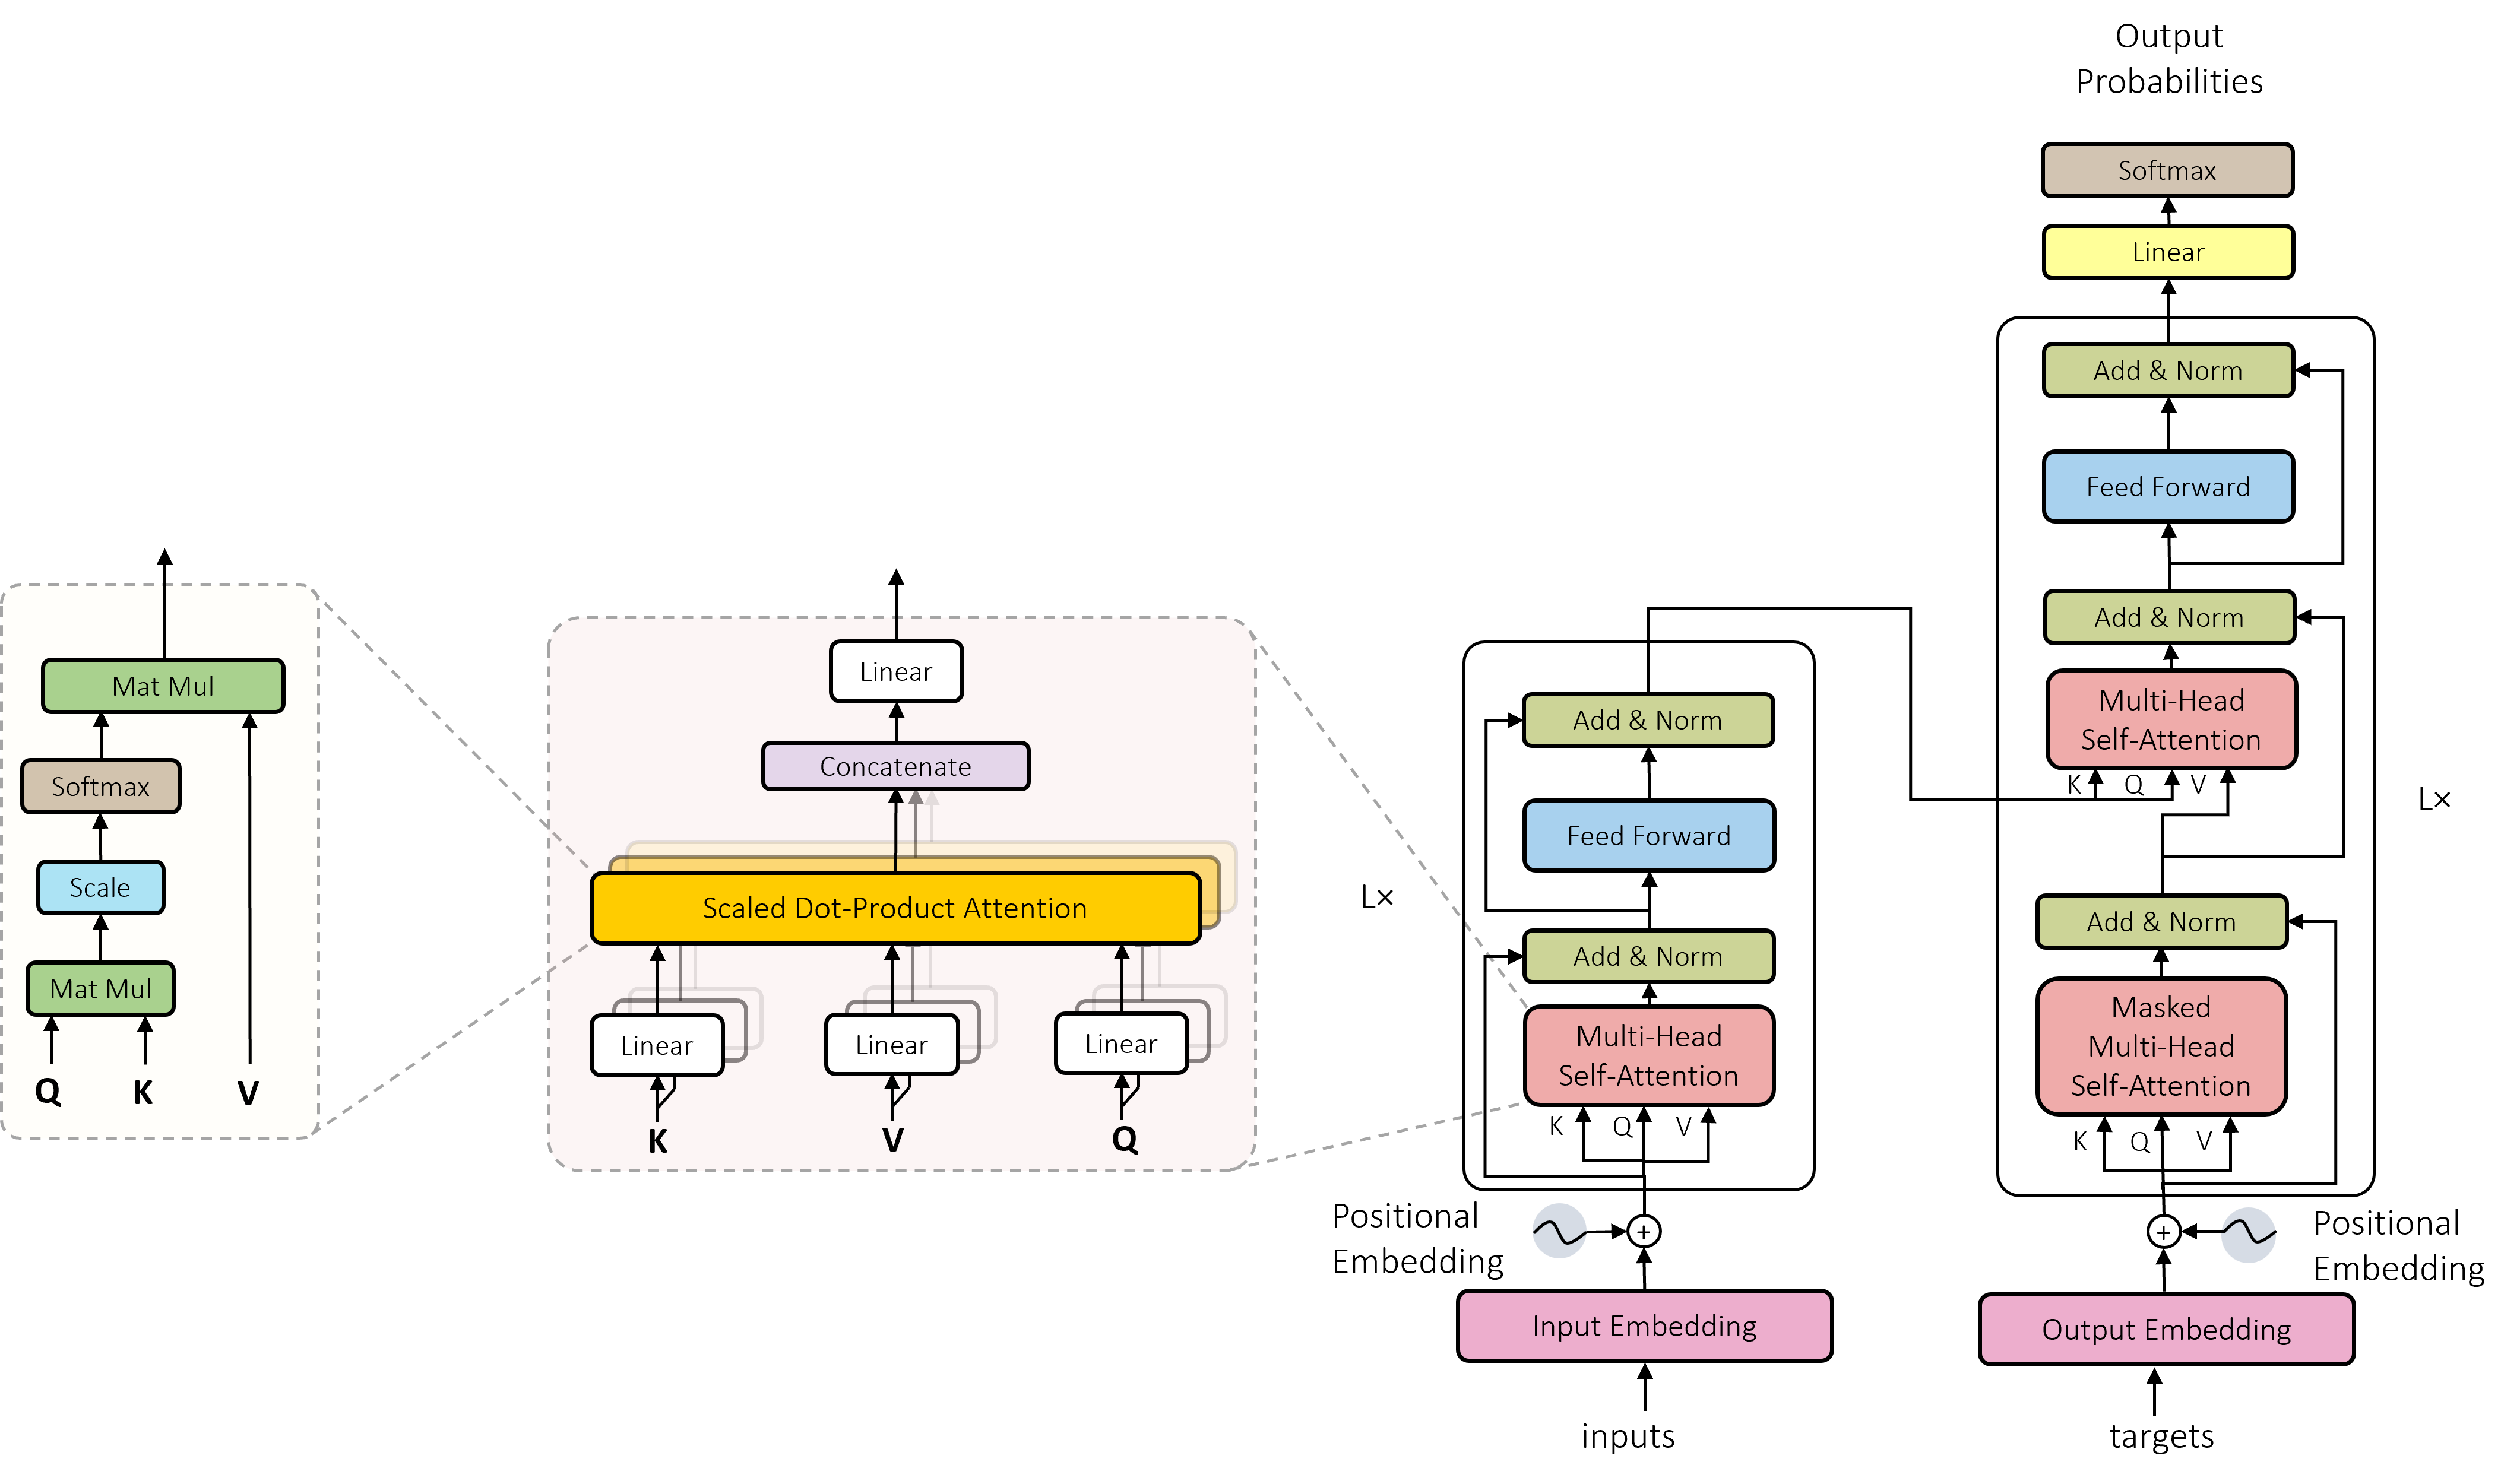
\includegraphics[width=\textwidth]{classical_transformer}
    \end{center}
    \caption{Own drawing inspired by \textcite{daiTransformerXLAttentiveLanguage2019}}
  \end{figure}
\end{landscape}

\subsubsection{Token Embedding}\label{sec:token-embeddings}

\subsubsection{Positional Encoding}\label{sec:positional-encoding}

\subsubsection{Attention}\label{sec:attention}

% \begin{equation}
%   \t{softmax}( \m{A})[t_\mathrm{z}, t_\mathrm{x}] ~:=~ \frac{\exp A[t_\mathrm{z},t_\mathrm{x}]}{ \sum_{t} \exp A[t,t_\mathrm{x}]},
% \end{equation}
% \begin{equation}\label{eq:mask}
%   \text{Mask}[t_\t{z},t_\t{x}] = \left\{{1~~~ \text{for bidirectional attention} 
%                                  \atop [\![t_\t{z}\!≤\!t_\t{x}]\!]~~ \text{for unidirectional att.}}\right.
% \end{equation}

% %-------------------------------%
% \begin{algorithm}[h] % Attention
% %-------------------------------%
%   \caption{$\m{\tilde V}\gets$~\texttt{Attention}$(\m{X},\m{Z}|\bmcWqkv,\text{Mask})$}
%   \label{algo:attention}
%   \KwIn{$\m{X}\in\mathbb{R}^{d_\t{x}\times\ell_\t{x}}, \m{Z}\in\mathbb{R}^{d_\t{z}\times\ell_\t{z}}$, vector representations of primary and context  sequence.}
%   \KwOut{$\m{\tilde V}\in\mathbb{R}^{d_\t{out}\times\ell_\t{x}} $, updated representations of tokens in $\m{X}$, folding in information from tokens in $\m{Z}$.}
%   \KwParam{$\bmcWqkv$ consisting of: 
%           $\m{W_q}\in\mathbb{R}^{d_\t{attn}\times d_\t{x}}$, $\v{b_q}\in\mathbb{R}^{d_\t{attn}}$
%            $\m{W_k}\in\mathbb{R}^{d_\t{attn}\times d_\t{z}}$, $\v{b_k}\in\mathbb{R}^{d_\t{attn}}$
%            $\m{W_v}\in\mathbb{R}^{d_\t{out}\times d_\t{z}}$, ~$\v{b_v}\in\mathbb{R}^{d_\t{out}}$.}
%   \KwHyper{Mask$\in\!\!\{0,\!1\}^{\ell_\t{z}\times\ell_\t{x}}$} %$\uparrow$\eqref{eq:mask}}
%   %%%%%%%%%%%%%%%%%%%%%%%%%%%%%%%%%%%%%%%%%%%%%%%%%%%%%%
%   $\m{Q} \gets \m{W_q} \m{X} + \v{b_q} \v{1}^\intercal$ ~ [\![$\m{Q}\t{uery}\in\mathbb{R}^{d_\t{attn}\times\ell_\t{x}}$]\!] \;
%   $\m{K} \gets \m{W_k} \m{Z} + \v{b_k} \v{1}^\intercal$ ~ [\![$\m{K}\t{ey}\in\mathbb{R}^{d_\t{attn}\times\ell_\t{z}}$]\!] \;
%   $\m{V} \gets \m{W_v} \m{Z} + \v{b_v} \v{1}^\intercal$ ~ [\![$\m{V}\t{alue}\in\mathbb{R}^{d_\t{out}\times\ell_\t{z}}$]\!] \;
%   $\m{S} \gets \m{K}^\intercal \m{Q}$ ~ [\![$\m{S}\t{core}\in\mathbb{R}^{\ell_\t{z}\times\ell_\t{x}}$]\!] \;
%   $\forall t_\t{z}, t_\t{x},$ if $\neg$Mask$[t_\t{z},t_\t{x}]$ then $S[t_\t{z},t_\t{x}] \gets -\infty  $ \;
%   \Return $\m{\tilde V} = \m{V}\cdot \t{softmax}\left( \m{S} / \sqrt{d_\t{attn}} \right)$    
% \end{algorithm}


\subsubsection{Position-wise Feed-Forward Networks}\label{sec:position-wise-ffn}

\subsubsection{Residual Connections}\label{sec:residual-connections}

\subsubsection{Layer Normalization}\label{sec:layer-norm}

\subsection{Transformer Networks For Tabular Data}\label{sec:tabular-transformer}

\subsubsection{Tabular Embeddings}\label{sec:tabular-embeddings}

\subsubsection{TabTransformer}\label{sec:tabtransformer}

\subsubsection{FTTransformer}\label{sec:fttransformer}


\newpage
\section{Semi-Supervised Approaches (8~p)}\label{sec:semi-supervised-approaches}

\subsection{Selection of Approaches (2~p)}\label{sec:selection-of-approaches-1}

\subsection{Extensions to Gradient Boosted
  Trees (2~p)}\label{sec:extensions-to-gradient-boosted-trees}

\subsection{Extensions to TabTransformer (2~p)}\label{sec:extensions-to-tabtransformer}

\subsection{Extensions to FTTransformer (2~p)}\label{sec:extensions-to-fttransformer}


\newpage
\section{Empirical Study (19.5~p)}\label{sec:empirical-study}

\subsection{Environment (0.5~p)}\label{sec:environment}

\subsection{Data and Data Preparation (6 p)}\label{sec:data-and-data-preparation}

\subsubsection{ISE Data Set (0.5~p)}\label{sec:ise-data-set}

\subsubsection{CBOE Data Set (0.5~p)}\label{sec:cboe-data-set}

\subsubsection{Exploratory Data Analysis (2~p)}\label{sec:exploratory-data-analysis}

\subsubsection{Data Pre-Processing (1~p)}\label{sec:data-preprocessing}

\subsubsection{Feature Engineering (1.5~p)}\label{sec:feature-engineering}

\subsubsection{Train-Test Split (0.5~p)}\label{sec:train-test-split}

\subsection{Training and Tuning (10~p)}\label{sec:training-and-tuning}

\subsubsection{Training of Supervised
  Models (4~p)}\label{sec:training-of-supervised-models}


\subsubsection{Training of Semi-Supervised
  Models (4~p)}\label{sec:training-of-semi-supervised-models}


\subsubsection{Hyperparameter Tuning (2~p)}\label{sec:hyperparameter-tuning}


\subsection{Evaluation (3~p)}\label{sec:evaluation}

\subsubsection{Feature Importance
  Measure (2~p)}\label{sec:feature-importance-measure}

\subsubsection{Evaluation Metric (1~p)}\label{sec:evaluation-metric}

\newpage
\section{Results (12~p)}\label{sec:results}

\subsection{Results of Supervised
  Models (2~p)}\label{sec:results-of-supervised-models}

\subsection{Results of Semi-Supervised
  Models (2~p)}\label{sec:results-of-semi-supervised-models}

\subsection{Robustness of Results (3~p)}\label{sec:robustness-checks}

\subsection{Feature Importance (3~p)}\label{sec:feature-importance}

\subsection{Ablation Study of Models (2~p)}\label{sec:ablation-study}

\newpage
\section{Application in Transaction Cost Estimation (optional)}\label{sec:application}
\subsection{Simulation Setup (optional)}\label{sec:simulation-setup}
\subsection{Simulation Results (optional)}\label{sec:simulation-results}

\newpage
\section{Discussion (3~p)}\label{sec:discussion}

\newpage
\section{Conclusion (2~p)}\label{sec:conclusion}

\newpage
\section{Outlook (0.5~p=67.5~p)}\label{sec:outlook}

